
\section{Anisotropías  considerando el peso de los hexágonos}

\subsubsection{Comparando los pesos en sidérea, solar y antisiderea.}


La idea que tengo sobre el pico en ambos gráficos es algo en la cantidad de hexagonos, algún periodo donde se apagó la mitad del observatorio o algo así.



\subsection{Variación de los pesos en función de la ascensión recta}
En las figuras de esta sección se muestran el análisis en ascensión recta para los eventos de observatorio considerando las variaciones de la exposición. 
Los mismos se hicieron en el mismo intervalo de tiempo para poder compararlos entre sí. Elegí el rango presentado en la Tabla \ref{rango_corto}  porque en el mismo se encuentran todos los eventos filtrados por energía, por bad period, por reconstrucción correcta, etc. El rango empieza en el 2013 porque la última versión del archivo de todos los disparos empezó a registrarse desde el  1 de Julio del 2013 a las 12:01:08 GMT (1372680068) hasta el  1 de enero del 2020 a las 11:59:43 (1577879983). Mientras que el archivo del disparo estándar va desde el 01 de enero del 2004.

	\begin{table}[H]
	\centering
		\begin{tabular}{c|c|c|c}
	 		& UTC 			& Fecha		 	&  Hora GMT  \\ \hline
	Inicio	& 1372699409	&2013-07-01 	&17:23:29		\\
	Final 	& 1577825634	&2019-12-31 	&20:53:54		\\
		\end{tabular}
	\caption{Rango de tiempo considerando todos los disparos} 	\label{rango_corto}
	\end{table}


\subsubsection{Energía entre 1\,EeV y 2\,EeV}

Para este caso utilizamos el archivo con todos los disparos en el rango de energía $1\,$ EeV - $2\,$EeV donde se tiene $1\,321\,702$ eventos.

\begin{figure}[H]
	\centering
	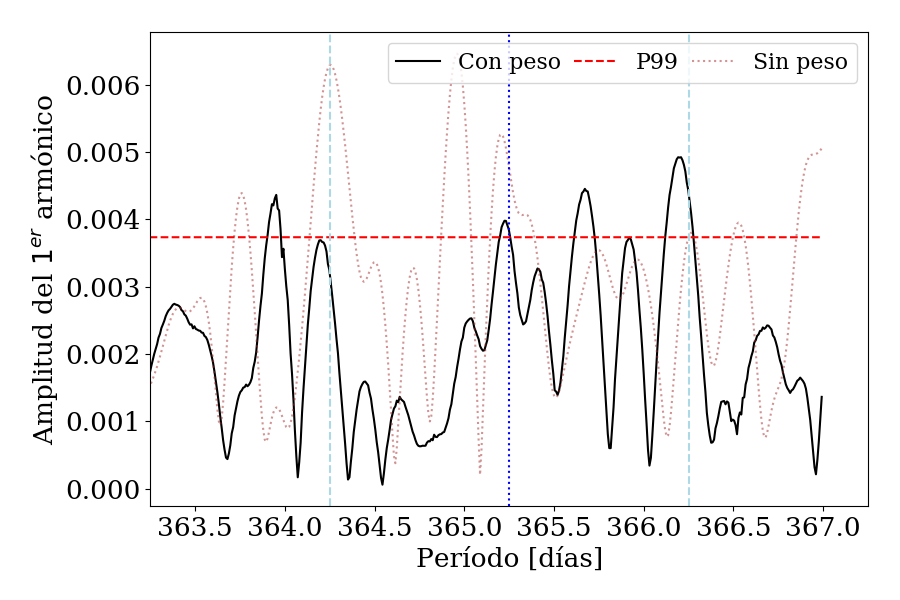
\includegraphics[width=0.5\textwidth]{Graficos/2019_AllTriggers_1_2_EeV_con_vs_sin_peso.png}
	\caption{Todos los disparos: entre 1 EeV y 2 EeV, entre 2013-2019}
	\label{fig:12w}
\end{figure}
%fig


La siguiente tabla se había calculado usando la formula 

\begin{equation}
	\tilde \alpha = 2\pi \frac{t_i}{T_x} +\alpha_i - \alpha^0
\end{equation}
donde $\alpha_i$ y $\alpha^o$ con las RA del evento y del cenit del observatorio.

	\begin{table}[H]
	\centering
		\begin{tabular}{c|c}
	 		&  2013-2019 (Con peso)	 \\ \hline
	Fase		& 	306.611				 \\
	$r$ 		&  0.00440897			\\
	$r_{99}$ 	&  0.00373348			\\
	$P(\tilde r)$ 	    & 	0.162485	\%	 \\
		\end{tabular}
	\caption{Rango de tiempo considerando todos los disparos} 	\label{rango_corto}
	\end{table}


\subsubsection{Energía entre 2\,EeV y 4\,EeV}

Para este caso utilizamos los eventos del archivo con todos los disparos con energía entre $2\,$ EeV - $4\,$EeV, donde se encontraron $288\,444$ eventos.
\begin{figure}[H]
	\centering
	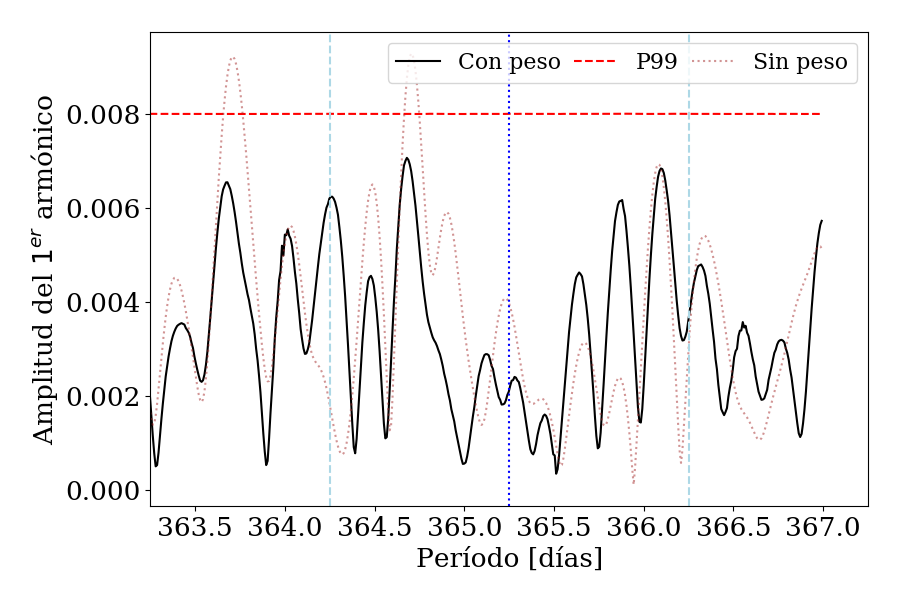
\includegraphics[width=0.5\textwidth]{Graficos/2019_AllTriggers_2_4_EeV_con_vs_sin_peso.png}
	\caption{Todos los disparos: entre 2 EeV y 4 EeV, entre 2013-2019}
	\label{fig:24w}
\end{figure}

En la Fig.\,\ref{fig:24w} no se ve ningún pico por encima de  percentil 99.


\subsubsection{Energía entre 4\,EeV y 8\,EeV}

A partir de $3\,$EeV el disparo estándar tiene una eficiencia del $100\%$. Entonces para este  intervalo de energías,  utilizamos el archivo con el disparo estandar.

\begin{figure}[H]
	\centering
	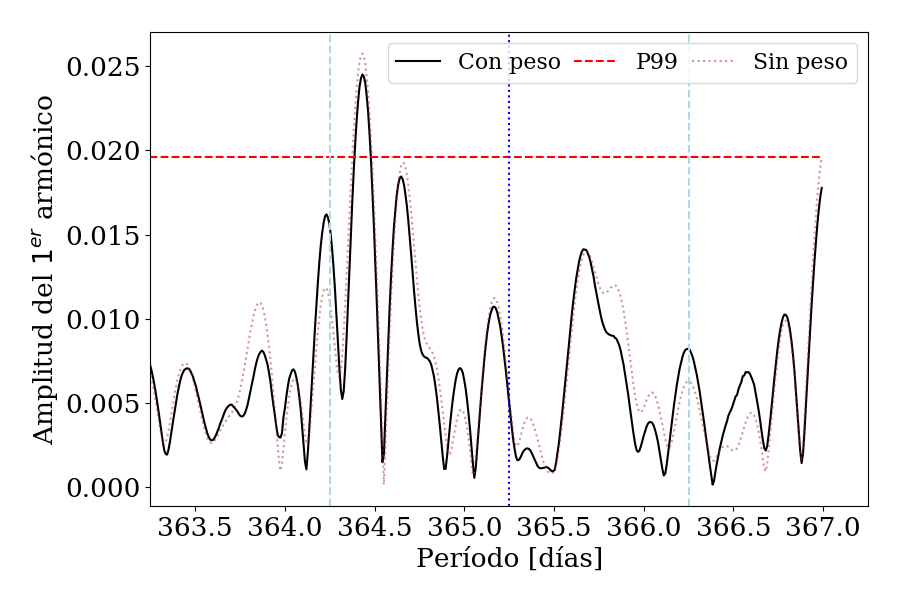
\includegraphics[width=0.5\textwidth]{Graficos/2019_Main_Array_4_8_EeV_con_vs_sin_peso.png}
	\caption{Disparos estándar: entre 4 EeV y 8 EeV, entre 2013-2019}
	\label{fig:48w}
\end{figure}
%fig

\subsubsection{Energía sobre 8\,EeV}

Para este caso utilizamos el archivo con el disparo estandar

\begin{figure}[H]
	\centering
	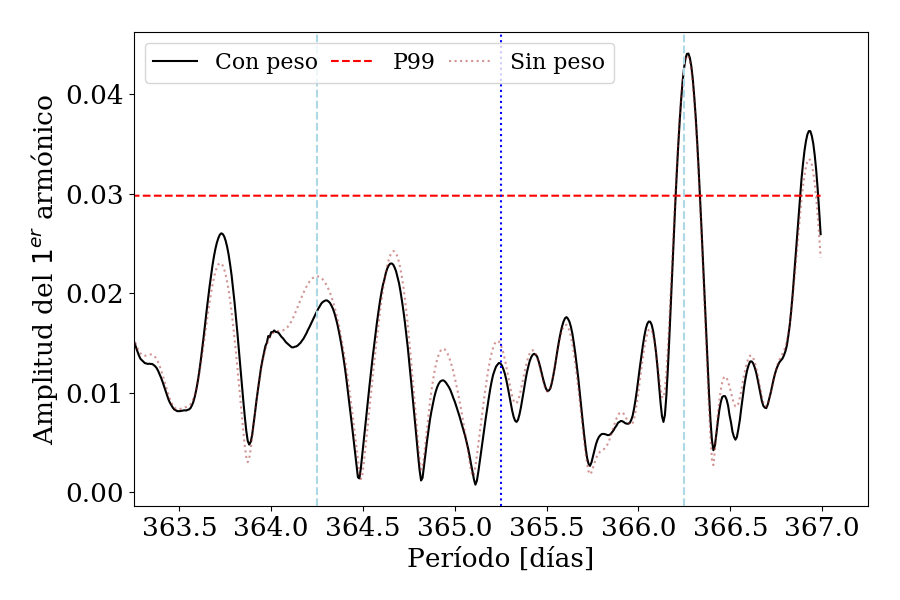
\includegraphics[width=0.5\textwidth]{Graficos/2019_Main_Array_8_EeV_con_vs_sin_peso.png}
	\caption{Disparos estándar: encima de 8 EeV, entre 2013-2019}
	\label{fig:8w}
\end{figure}
%fig




\subsection{Ampliando el rango de tiempo para el archivo del disparo estándar}

Amplié el rango de tiempo para poder compararlo con los gráficos anteriores, ya que se espera que mientras mayor sea el rango de tiempo los efectos espúreos disminuyen.

	\begin{table}[H]
	\centering
		\begin{tabular}{c|c|c|c}
	 		& UTC 			& Fecha		 	&  Hora GMT  \\ \hline
	Inicio	& 1104537600	&2005-01-01 	&00:00:00		\\
	Final 	& 1577825634	&2019-12-31 	&20:53:54		\\
		\end{tabular}
	\end{table}


\subsubsection{Energía entre 4\,EeV y 8\,EeV}

\begin{figure}[H]
	\centering
	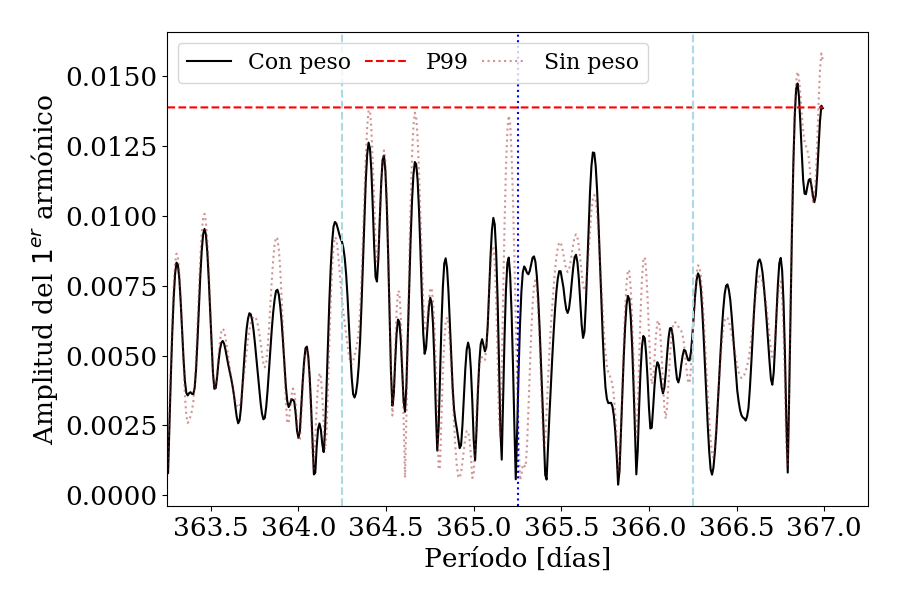
\includegraphics[width=0.5\textwidth]{Graficos/2019_Main_Array_4_8_EeV_con_vs_sin_peso_extended.png}
	\caption{Disparos estándar: entre 4 EeV y 8 EeV extendiendo el rango hasta el 2005}
	\label{fig:48w_extended}
\end{figure}
%fig

\subsubsection{Energía sobre 8\,EeV}


\begin{figure}[H]
	\centering
	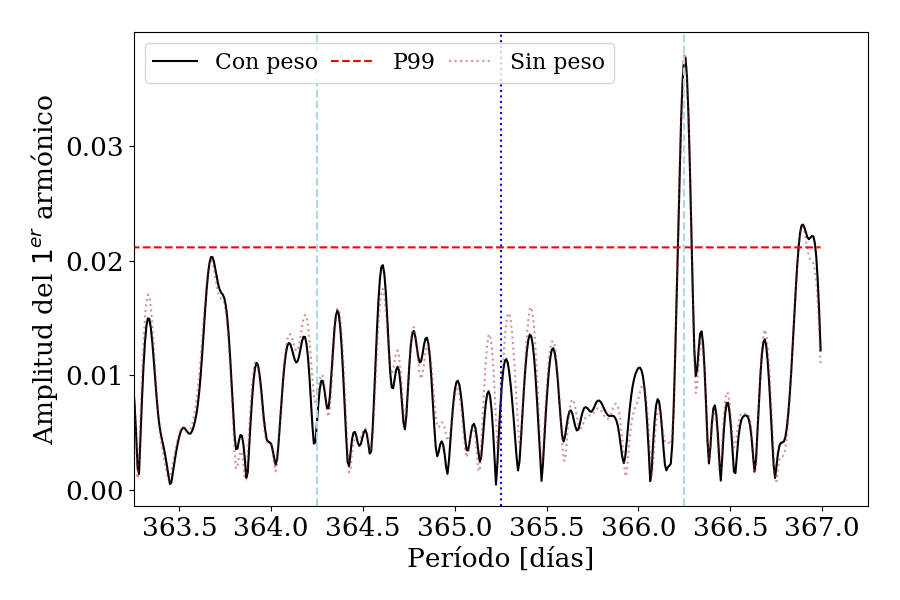
\includegraphics[width=0.5\textwidth]{Graficos/2019_Main_Array_8_EeV_con_vs_sin_peso_extended.png}
	\caption{Disparos estándar: encima de 8 EeV extendiendo el rango hasta el 2005}
	\label{fig:8w_extended}
\end{figure}
%fig